\subsection{Martina Ravaioli}
\subsubsection{caselle speciali}

\textbf{Problema}\newline
Nel gioco di monopoli è necessario creare delle carte speciali ognuna con il proprio effetto specifico. La creazione di tali carte può portare a proliferazione di classi e difficoltà di manutenzione.\newline
\textbf{Soluzione}\newline
In questa soluzione si utilizza il Factory Pattern per centralizzare la creazione all’interno della classe \texttt{SpecialFactory} e nasconderne i dettagli implementativi.
La factory di speciali ritorna una carta speciale con un effetto specifico, la creazione dell’effetto la delega a sua volta ad una factory di effetti (\texttt{EffectFactory}).
Limitando la creazione alla factory si evita di violare il principio DRY(Don’t Repeat Yourself) per la ripetizione del codice e si rende più semplice l’aggiunta di altre eventuali carte  in quanto basta aggiungere un metodo alla classe SpecialFactory promuovendo il SRP (Single Responsibility Principle)

\begin{figure}[H]
    \centering
    \makebox[1\textwidth]{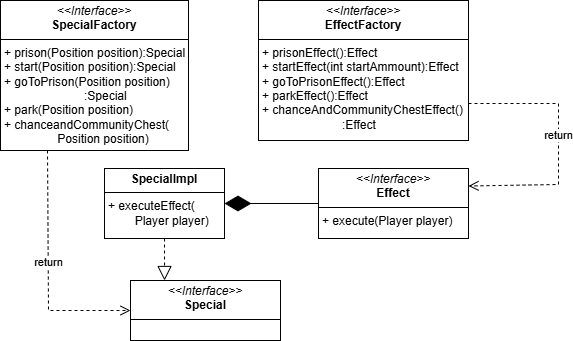
\includegraphics[width=0.75\textwidth]{img/martina/specialsUML.png}}
    \caption{Schema UML del pattern factory. SpecialFactory nasconde dentro ogni metdo la creazione delle relative carte che a loro volta delegano la creazione degli effetti al relativo metodo in Effect Factory}
    \label{img:ArchitectureDiagram-Pagina-4}
\end{figure}

\textbf{Problema}\newline
Nel gioco ci sono le società, delle proprietà che quando ci arrivi sopra l’affitto da pagare è il tiro del dado moltiplicato per un certo fattore dato da quante società si possiedono. 
La creazione di una carta a sé può portare a duplicazione di codice. \newline
\textbf{Soluzione}\newline
in questa soluzione mi sono ricondotta al pattern decorator, per composizione un \texttt{SpecialTitleDeed} ha un (\texttt{BaseTitleDeed}) a cui modifica le opzioni di affitto attraverso vari fattori moltiplicativi.
Così facendo non ci sarà duplicazione del codice implementativo delle proprietà normali con la sola variazione dell'affitto.
\begin{figure}[H]
    \centering
    \makebox[1\textwidth]{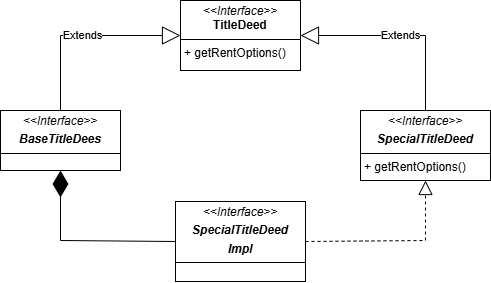
\includegraphics[width=0.75\textwidth]{img/martina/specialPropertyUML.png}}
    \caption{Gli SpecialTitleDeed fanno override del metodo getRentOptions}
    \label{img:ArchitectureDiagram-Pagina-3}
\end{figure}

\subsubsection{Player}

\textbf{Problema}\newline
Nel gioco i giocatori devono poter essere messi in prigione o nel parcheggio e di conseguenza perdere l’abilità di giocare un numero predefinito di turni. 
Nel caso del parcheggio viene saltato solo il turno successivo ma non c’è modo di evitare questo effetto.
Nel caso della prigione i turni che vengono saltati sono 3 ma il giocatore ha la possibilità, prima di perdere il turno, di tirare i dadi per provare ad uscire di prigione facendo un tiro di almeno 2 numeri uguali.
Per poter creare dei player che possono essere messi in prigione ma non nel parcheggio e viceversa si dovrebbero creare tutte le possibili combinazioni e dunque duplicare molto codice.\newline
\textbf{Soluzione}\newline
per risolvere questo problema mi sono ricondotta al pattern decorator. 
Nell'implementazione base del player (\texttt{PlayerImpl}) sono presenti tutti i metodi per gestire questi due eventi ma la loro implementazione è delegata a classi specializzate che verranno usate per decorare il player all’inizio del gioco (\texttt{ParkablePlayer, PrisonablePlayer}). 
In questo modo si mantengono in classi separate le implementazioni dei metodi per la gestione di questi due problemi e si rende il gioco più adattivo nel caso in cui si volesse giocare una versione dove l’effetto della prigione o del parcheggio risultino disabilitati

\begin{figure}[H]
    \centering
    \makebox[1\textwidth]{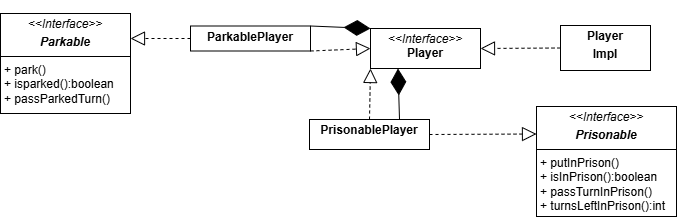
\includegraphics[width=0.75\textwidth]{img/martina/parkableAndPrisonableUML.png}}
    \caption{Prisonable e parkable fanno entrambi override dei metodi nelle rispettive interfacce}
    \label{img:ArchitectureDiagram-Pagina-2}
\end{figure}

\subsubsection{Imprevisti e Probabilità}

\textbf{Problema}\newline
Nel gioco ci sono delle caselle speciali di tipo imprevisto o probabilità che fanno pescare una carta da uno fra due mazzi per poi svolgere le azioni presenti su quella carta.
Le azioni sono una composizione di altre azioni più semplici che hanno ripercussioni sul turno del giocatore.
Scrivere tutto l’effetto all’interno della classe carta porterebbe a rendere il codice poco espandibile.

\textbf{Soluzione}\newline
Nella risoluzione di questo problema mi sono rifatta al pattern command. Ci sono due tipi di comandi che incapsulano il concetto di effetto, i comandi con più azioni da eseguire (\texttt{ComplexCommand}) e quelli che incapsulano una sola delle azioni di quelli composti \texttt{BaseCommand} estendono entrambi la stessa interfaccia. Quelli complessi  si salvano una lista di comandi base associati agli argomenti con cui devono essere eseguiti. 
L’interfaccia \texttt{command} ha solo il metodo execute che prende in ingresso il player che ha fatto attivare l’effetto e gli argomenti con cui quell’effetto deve essere attivato. 
Le carte imprevisto o probabilità si salveranno un comando complesso che verrà attivato quando viene pescata la carta.
\begin{figure}[H]
    \centering
    \makebox[1\textwidth]{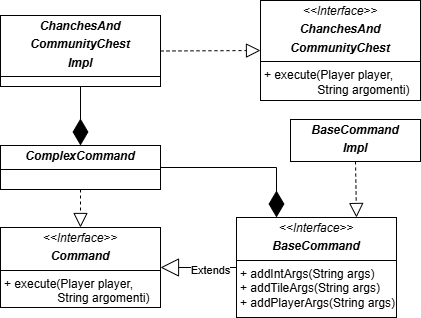
\includegraphics[width=0.75\textwidth]{img/martina/commandsUML.png}}
    \caption{schema UML della gestione dei comandi delle carte imprevisto e probabilità}
    \label{img:ArchitectureDiagram-Pagina-1}
\end{figure}

\textbf{Problema}\newline
La creazione dei comandi delle carte imprevisti può portare ad un enorme spreco di memoria e una grande proliferazione del codice visto che sono tanti effetti composti dalle stesse azioni base.  \newline
\textbf{Soluzione}\newline
Per alcune parti di questa soluzione mi sono ispirata al pattern interpreter ma per la maggior parte ho dovuto aggiungere parti per adattarla al problema. 
L’interpretazione dei comandi delle carte imprevisti e probabilità avviene su 4 livelli e prende le informazioni su come comporre i detti effetti da un file nella cartella di risorse. 
I 4 interpreter sono fatti per rendere più semplice e più vicina al linguaggio naturale la scrittura del file. 
Il primo interpreter (\texttt{DeckCreator}) prenderà dal file il blocco di informazioni che definisce l’intero effetto della carta e con quel blocco delega la creazione dell’effetto all’interpreter successivo. Una volta ottenuto l’effetto sotto forma di un \texttt{ComplexCommand} (Vedi soluzione sopra) creerà una nuova carta imprevisto-probabilità che una volta attivata eseguirà le istruzioni contenute dentro il comando. Dopo aver creato tutte le carte si occuperà di aggiungere il deck
Il secondo interpreter (\texttt{ComplexInterpreter}) ricevuto il blocco con tutto l’effetto lo scompone, riga per riga nelle varie azioni base previste, ogni riga viene a sua volta divisa in due parti. 
La prima parte viene passata all’interpreter successivo per sapere quale comando base usare, una volta ottenuto il tipo di comando base questo verrà memorizzato assieme alla seconda parte della stringa che verrà poi passata al metodo execute quando l’effetto dovrà essere eseguito.  
Il terzo interpreter (\texttt{BaseInterpreter}), attraverso un sistema di keyword univoche per ogni tipo di comando base, ritorna il riferimento al comando base relativo alla stringa passata dall’ interpreter precedente.
Il quarto interpreter (\texttt{ArgsInterpreter}) situato dentro ogni comando base, si attiva quando il comando viene eseguito e si occupa di elaborare la stringa con gli argomenti e aggiungerli nei vari campi per fare in modo che l’azione venga eseguita correttamente.
Per ogni tipo di comando base viene creato un solo oggetto contenente le istruzioni da eseguire, quando il terzo interpreter “crea” un nuovo comando base in realtà sta solamente indicando quale dei comandi già creati usare per eseguire l’azione desiderata.
Questo è fatto per evitare di creare una moltitudine di oggetti di tipo base command, tutti uguali tra loro tranne che per gli argomenti con cui vengono eseguiti.
\begin{figure}[H]
    \centering
    \makebox[1\textwidth]{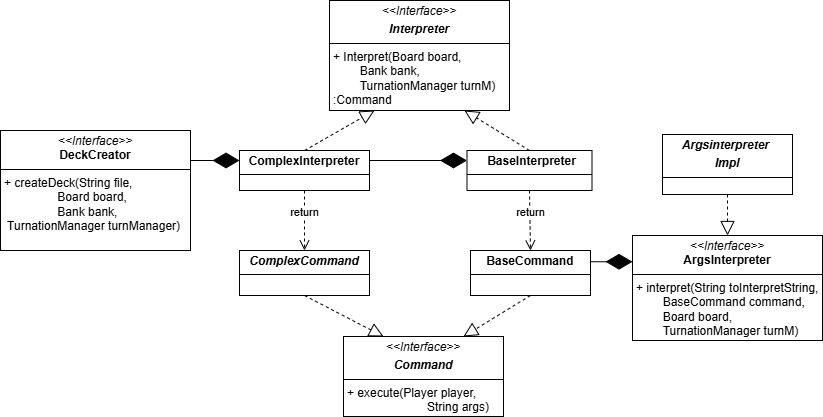
\includegraphics[width=1\textwidth]{img/martina/interpretersUML.png}}
    \caption{Schema UML degli interpreti a cascata per la creazione dei comanndi}
    \label{img:ArchitectureDiagram-Pagina-5}
\end{figure}
